\documentclass[10pt,a4paper,twocolumn]{article}
\usepackage[utf8]{inputenc}
\usepackage{amsmath}
\usepackage{amsfonts}
\usepackage{amssymb}
\usepackage{graphicx}
\usepackage{hyperref}
\usepackage{listings}
\usepackage{float}
\usepackage[dutch]{babel}
\author{Ruben Van Assche}
\graphicspath{ {../plots/} }
\title{Data Fitting - Oefening 5}
\date{\today}
\begin{document}
\maketitle
\section{Software}
Doorheen deze opgave heb ik gebruik gemaakt van GSL\footnote{\url{https://www.gnu.org/software/gsl/}}. Alle functies in deze opgave gebruikt komen dan ook uit de \texttt{\detokenize{gsl_interp}} workspace.
\section{Interpolerende Veelterm}
Voor het eerste deel van de opgave moest een interpolerende veelterm van graad 16 berekend worden dit betekent dat er 17 punten vereist zijn welke gegeven worden door: $x_{i},i = 0,\hdots,16$ met onderlinge afstand $\frac{2}{16}$ waarbij $f(x) = arctan(x)$. Dit levert volgende resultaten op:
$$
\begin{tabular}{ l c r }
  X & Y\\
-1 & -0.785398163397448279\\
-0.875 & -0.7188299996216245269\\
-0.75 & -0.64350110879328437097\\
-0.625 & -0.55859931534356244143\\
-0.5 & -0.46364760900080614903\\
-0.375 & -0.35877067027057224502\\
-0.25 & -0.24497866312686414347\\
-0.125 & -0.12435499454676143816\\
0 & 0\\
0.125 & 0.12435499454676143816\\
0.25 & 0.24497866312686414347\\
0.375 & 0.35877067027057224502\\
0.5 & 0.46364760900080614903\\
0.625 & 0.55859931534356244143\\
0.75 & 0.64350110879328437097\\
0.875 & 0.7188299996216245269\\
1 & 0.785398163397448279\\
\end{tabular}
$$
Vervolgens genereren we een veelterm interpolant(\texttt{\detokenize{gsl_interp_polynomial}}) d.m.v. de \texttt{\detokenize{gsl_spline_init}} functie. Hierna berekenen we op het interval $[-1, 1]$ x waarden met stappen van $0.01$. Bij elke stap evalueren we dan via \texttt{\detokenize{gsl_spline_eval}} de interpolant voor de x-waarde in het interval $[-1,1]$. Om de oplossing te checken bereken we voor elke x-waarde ook $arctan(x)$ zodat we de foutenkromme $(P(x) - arctan(x)/arctan(x)$ kunnen berekenen. Deze data wordt weg geschreven naar verschillende bestanden zodat er grafieken van gemaakt kunnen worden.

\subsection{Bevindingen}
Ten eerste kijken we naar een plot van de interpolant en de originele functie $arctan(x)$. Wat meteen opvalt is dat de interpolant de originele functie benadert(er zijn geen twee verschillende functies te onderscheiden op de plot).
\begin{figure}[h]
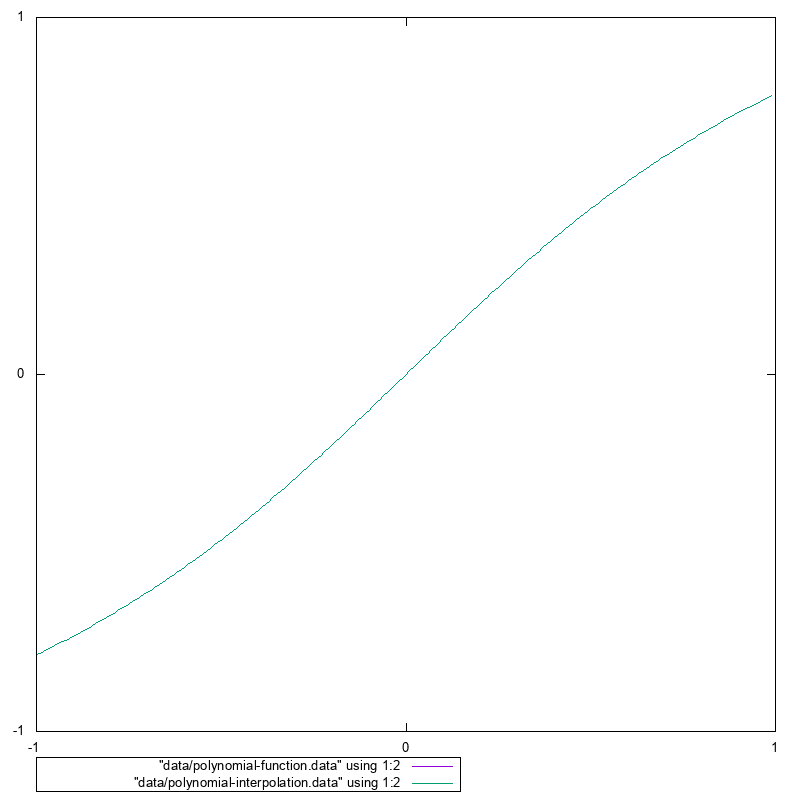
\includegraphics[width=0.5\textwidth]{polynomial}
\end{figure}
\newline
Gezien dat de interpolant zo goed als gelijk ligt met de oorspronkelijke functie verwachten we een foutenkromme met kleine fouten. We zien een duidelijke uitschieter rond 0(alhoewel de waarde exact in $x = 0$ gelijk aan 0 is).
\begin{figure}[h]
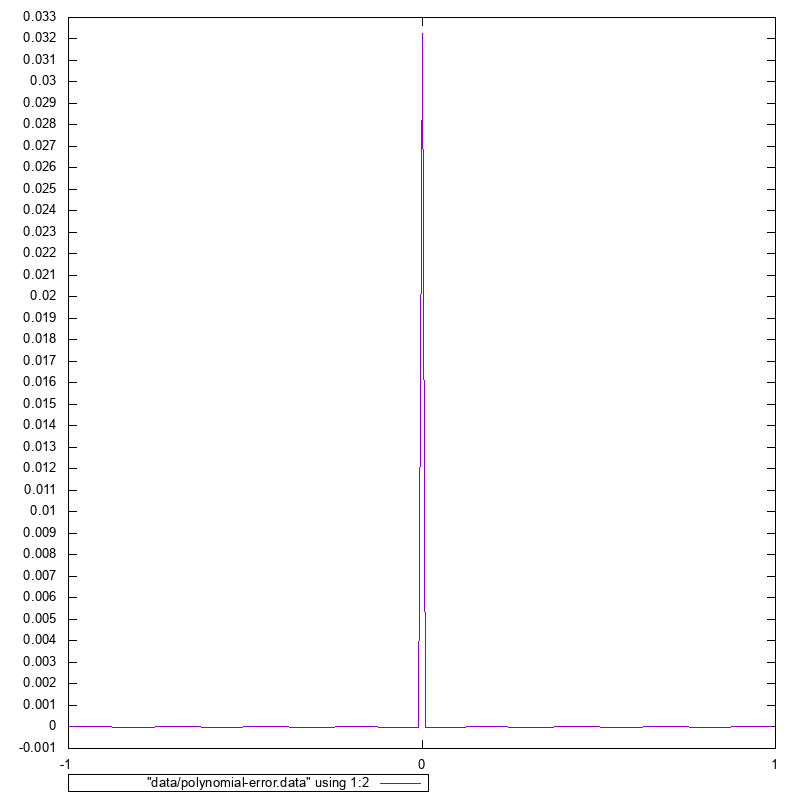
\includegraphics[width=0.4\textwidth]{polynomial-error}
\end{figure}
\newline
Wanneer we inzoomen op de grafiek(ik heb even het uitschieter nulpunt vervangen door (0,0) voor een beter beeld) zien we duidelijk het Runghe fenomeen optreden. Dit komt omdat we een polynomiale veelterm van graad 16 hebben. Er ontstaan duidelijk oscillaties aan de buitenkanten van het interval. Deze oscillaties zijn vrij klein dus gaan zoals eerder gezegd niet veel effect hebben op de interpolerende functie t.o.v. de originele functie.
\begin{figure}[h]
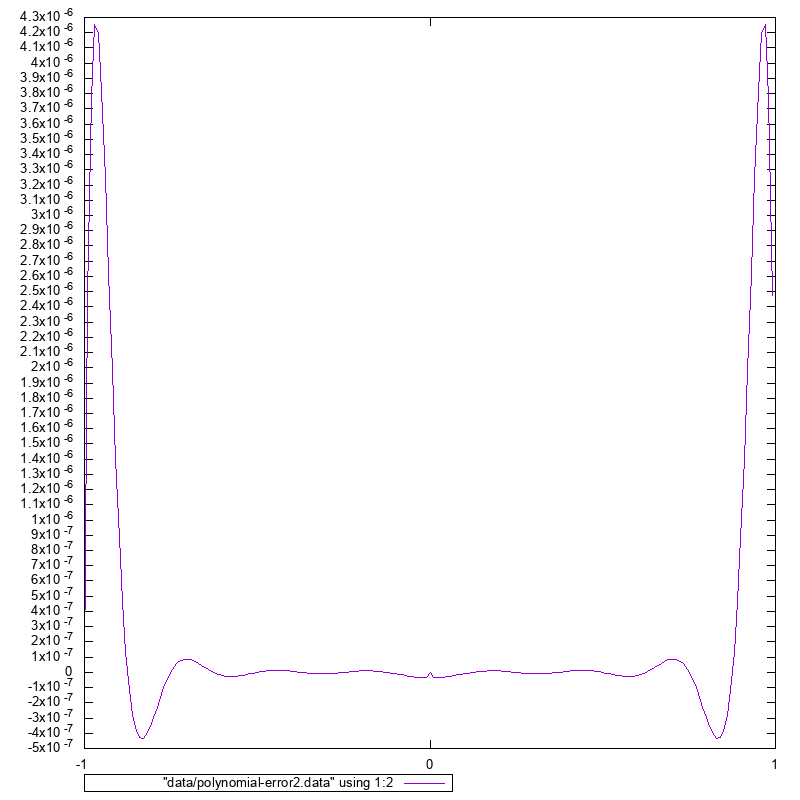
\includegraphics[width=0.40\textwidth]{polynomial-error2}
\end{figure}
\newline
Wat natuurlijk zeer belangrijk is bij een interpolerende functie, is dat deze door de gegeven punten koppels $(x_{i}, f(x_{i})$  gaan. Wanneer we volgende grafiek bekijken zien we dat 6 van de puntenkoppels niet exact hetzelfde zijn als de originele koppels. Gelukkig zitten we hier met relatief kleine fouten($10^{-16}$) wat niet zeer dramatisch is.
\begin{figure}[h]
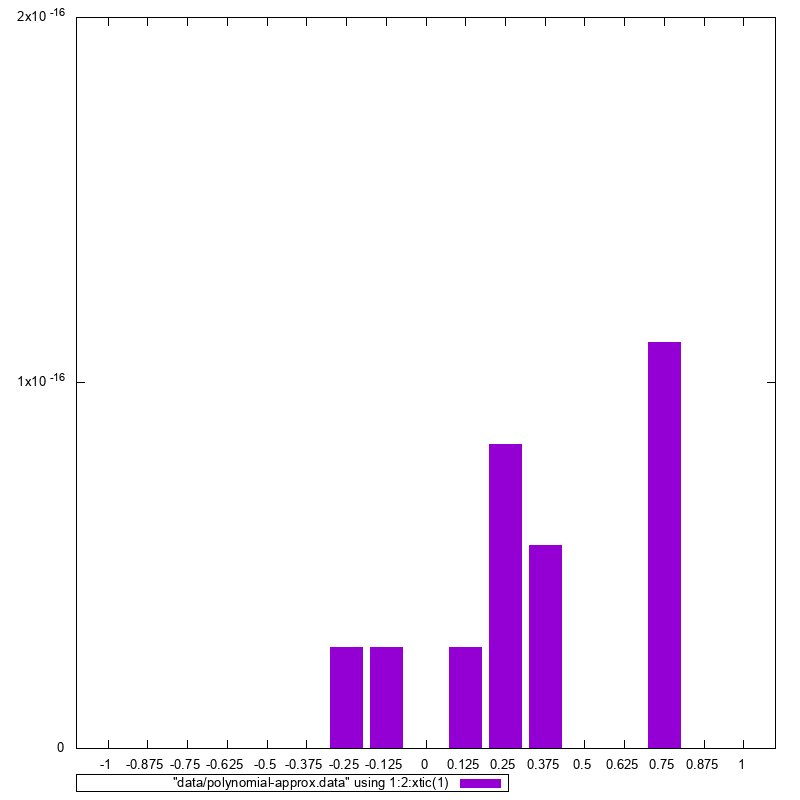
\includegraphics[width=0.4\textwidth]{polynomial-approx}
\end{figure}
\newline
\section{Mock-Chebyshev Polynomial}
Bij deze interpolatie methode gaan we eerst een equidistant grid generen om vervolgens 17 punten te selecteren die dicht liggen bij de Chebyshev punten. Deze punten worden gegeven door : $t_{i} = cos((2i + 1)\pi/34)$ waarbij $i = 0,\hdots,16$. Vervolgens generen we een grid met een bepaalde spacing ertussen(bijvoorbeeld 0.1, elk punt ligt 0.1 afstand van elkaar). Nu is ons doel de beste spacing te kiezen zodat de gegenereerde geïnterpoleerde functie zo goed mogelijk door de originele puntenkoppels lopen.
\subsection{Selecteren Punten}
Om de punten op het equidistante grid te selecteren als Mock-Chebyshev punten gebruiken we volgend algoritme : voor elk Mock-Chebyshev punt overlopen we alle punten in het equidistante grid en berekenen we de afstand tussen het Mock-Chebyshev punt en het equidistant punt. Het equidistante punt dat de kleinste afstand heeft wordt toegevoegd aan de set interpolatie punten en wordt verwijderd van het equidistante grid zodat het geen 2 keer wordt geselecteerd.
\subsection{Spacing kiezen}
Nu rest ons enkel nog een spacing te kiezen! Hiervoor berekenen we de geïnterpoleerde functie met een spacing van 0.0001 en berekenen deze telkens opnieuw door het toevoegen van stapjes van 0.0001 tot we 0.1 bereiken. Telkens bij deze berekening kijken we naar hoe goed de geïnterpoleerde functie door de gegevens punten koppels gaan. Het verschil met de gegeven punten koppels tellen we elke stap op en stellen we gelijk aan $goodness$. Op het einde nemen we de spacing waar $goodness$ minimaal is. Hieronder staat een tabel met waarden voor spacing en goodness waarbij we gebruik maken van stappen van 0.01(om het rapport niet te lang te maken). Deze waarden geven een goede impressie over hoe het verloop met kleinere spacingen gaat.
$$
\begin{tabular}{ l c r }
  Spacing & Goodness\\
0.01000 & 9.1185217707437793422\\
0.02000 & 9.1165830180332019239\\
0.02999 & 9.1111268851547571046\\
0.02999 & 9.1111268851547571046\\
0.02999 & 9.1111268851547571046\\
0.06000 & 9.0704190748879369721\\
0.07000 & 8.9158443749093247988\\
0.07000 & 8.9158443749093247988\\
0.08999 & 8.8075303794024506487\\
\end{tabular}
$$
Uiteindelijk bekomen we voor een spacing 0.095300000000001702793 een minimale goodness 8.3149805547451816068.
\subsection{Grid}
Wanneer we vervolgens naar het originele equidistant grid kijken.
\begin{figure}[H]
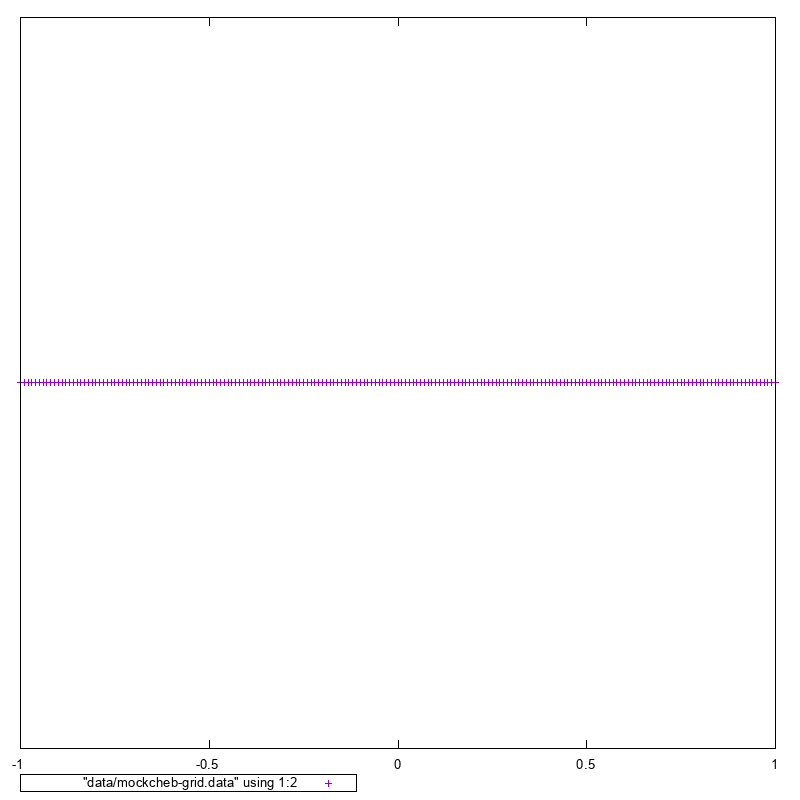
\includegraphics[width=0.4\textwidth]{mockcheb-gridPoints}
\end{figure}
En het Mock-Chebyshev grid, zien we dat de equidistante punten nu de Chebyshev punten benaderen!
\begin{figure}[H]
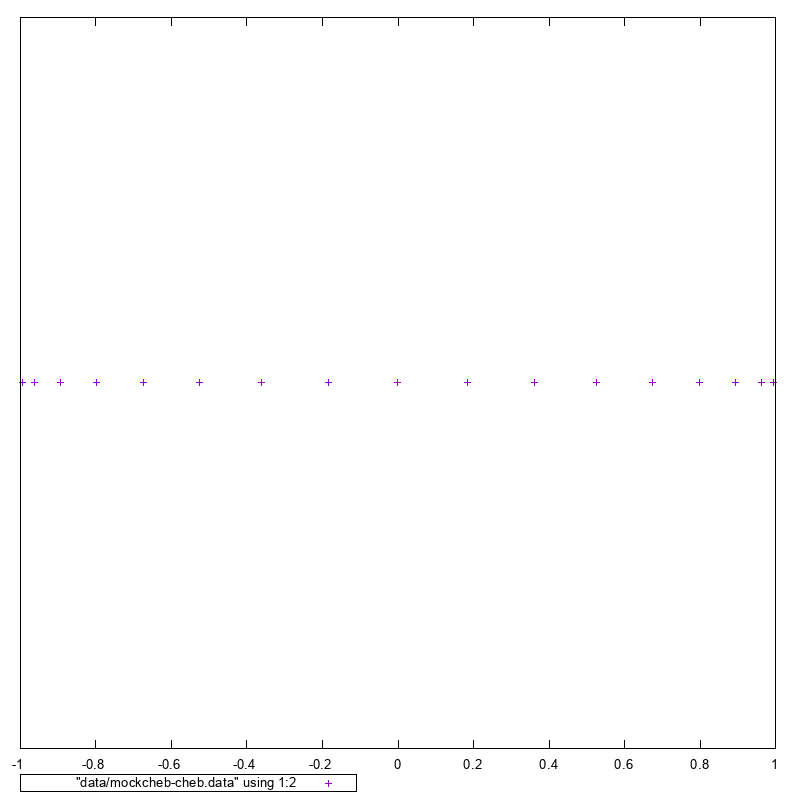
\includegraphics[width=0.4\textwidth]{mockcheb-chebPoints}
\end{figure}
Vervolgens kijken we naar een plot van de geïnterpoleerde en originele functie $fx) = arctan(x)$ en zien net als bij de "gewone" polynomische interpolatie dat dat beide krommen gelijk lopen.
\begin{figure}[H]
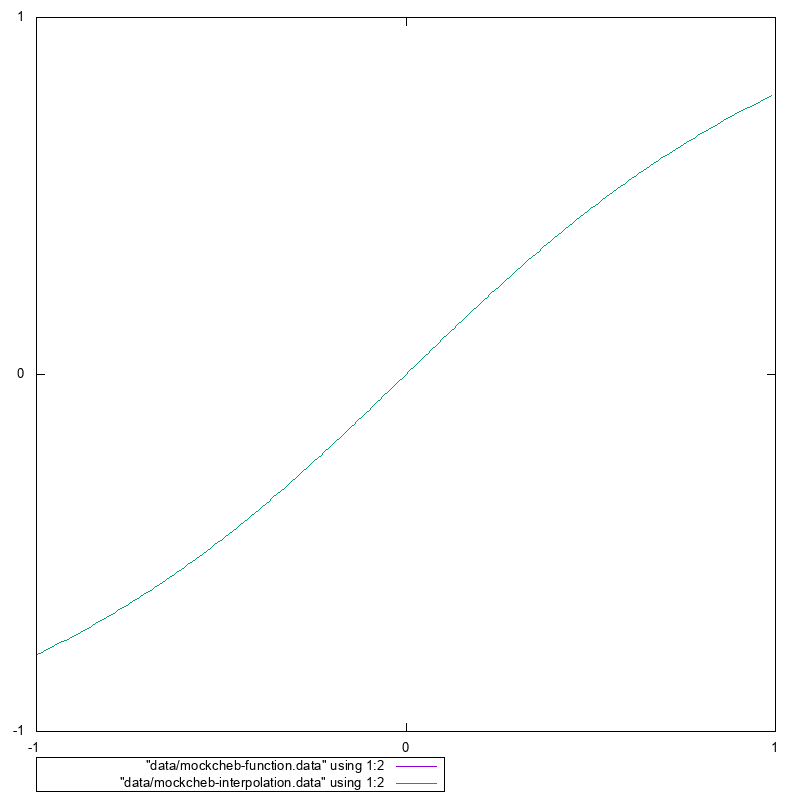
\includegraphics[width=0.4\textwidth]{mockcheb}
\end{figure}
De foutenkromme laat wel een verschil zien met de "gewone" polynomische interpolatie: ten eerste is de error kleiner geworden. Maar wat belangrijker is: het Runghe effect dat optrad bij de vorige interpolatie methode is meer "plat gedrukt". Het is nu gelijker verdeeld over de gehele kromme, er zijn dus geen specifieke uitschieters aan de uiteinden van het interval.
\begin{figure}[H]
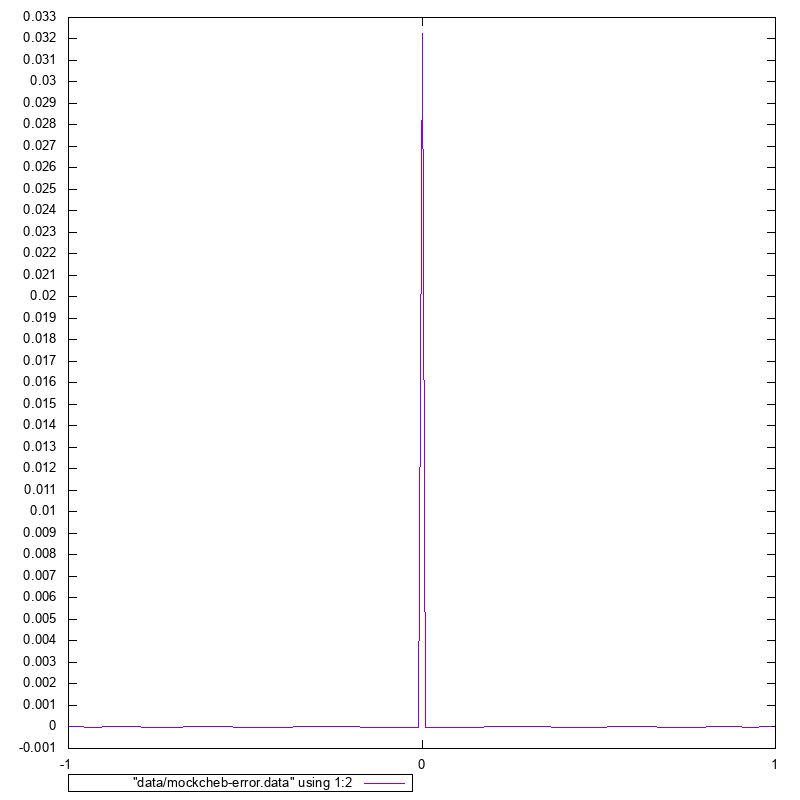
\includegraphics[width=0.4\textwidth]{mockcheb-error}
\end{figure}
Dan kijken we nog naar hoe goed deze methode door de gegevens puntenkoppels gaan:
\begin{figure}[H]
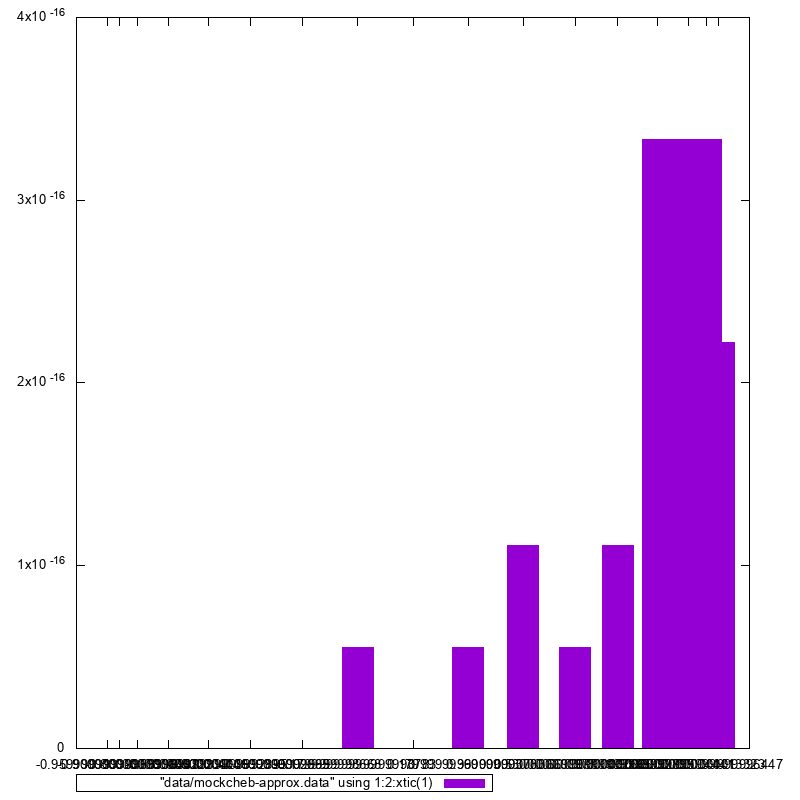
\includegraphics[width=0.4\textwidth]{mockcheb-approx}
\end{figure}
Wat opvalt: in tegenstelling tot de vorige methode is het aantal punten waarbij de geïnterpoleerde kromme niet door de originele puntenkoppels gaat groter geworden. En daar bijkomend: de afstand tussen de originele kromme en geïnterpoleerde kromme is voor de originele puntenkoppels groter geworden. Dit is dus niet de beste keuze als methode voor interpolatie.
\section{Spline}
Als laatste kijken we naar de natuurlijke kubische spline deze wordt in GSL gedefinieerd als \texttt{\detokenize{gsl_interp_cspline}} het verdere werk voor het genereren van de spline is gelijk aan de procedure beschreven in sectie 2.
\subsection{Bevindingen}
Wanneer we kijken naar een plot van de spline en de originele functie $f(x) = arctan(x)$ merken we in tegenstelling tot de andere interpolaties dat de geïnterpoleerde functie lichtjes afwijkt van de originele functie. 
\begin{figure}[H]
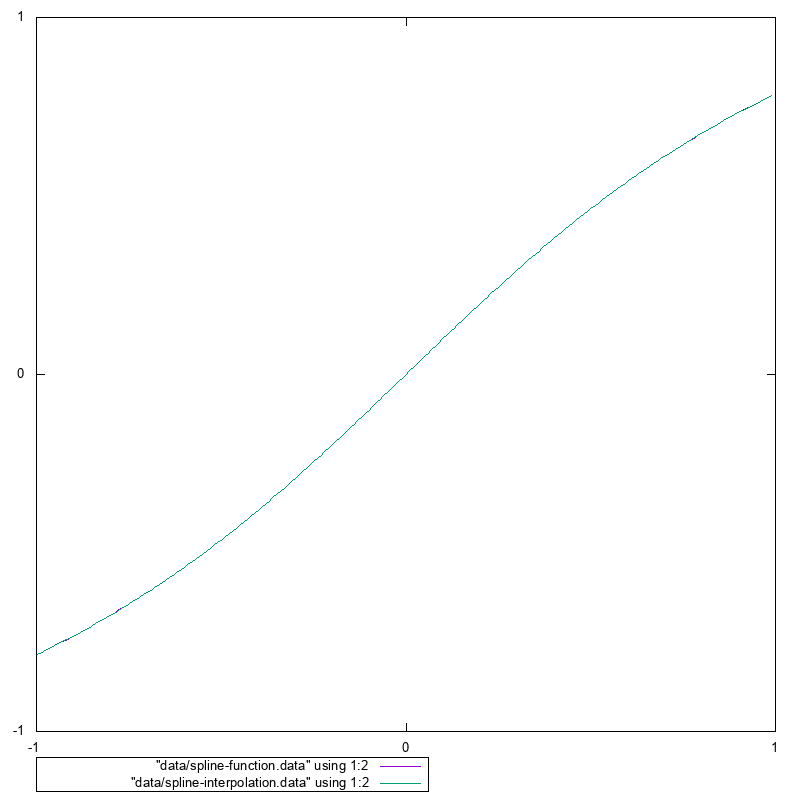
\includegraphics[width=0.4\textwidth]{spline}
\end{figure}
Dit vertaalt zich ook in de  geplotte foutenkromme: alhoewel we hier geen Runghe fenomeen zien(het voordeel van de spline). Valt er wel uit de data(\texttt{\detokenize{spline-error.data}}) op dat de fouten een stuk groter zijn($10^{-3}$) t.o.v. de polynomische interpolatie. Dit zorgt er dus voor dat de beide krommen op de vorige grafiek niet altijd even gelijk lopen.
\begin{figure}[H]
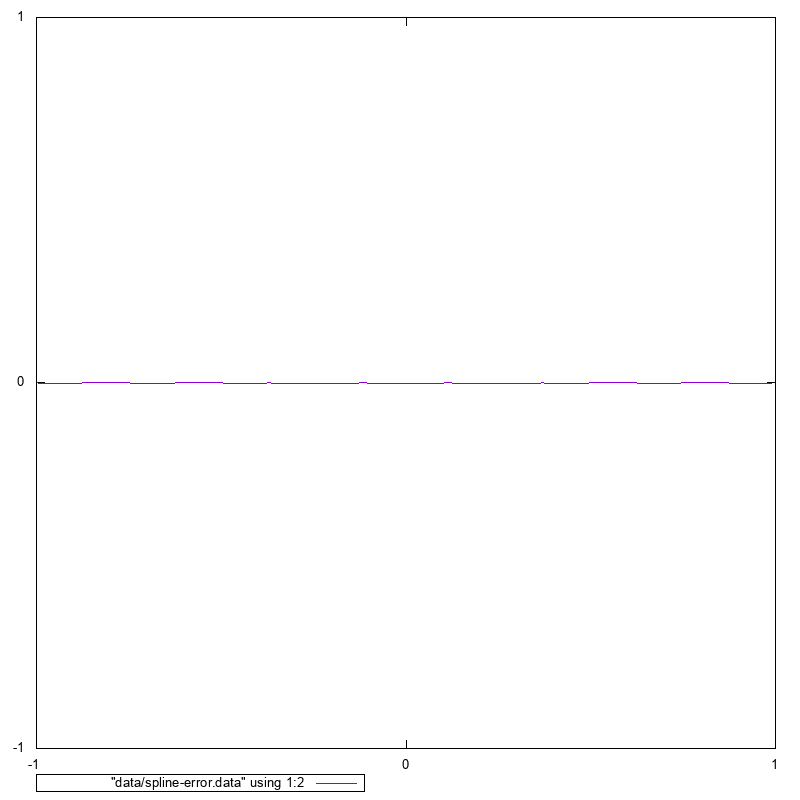
\includegraphics[width=0.4\textwidth]{spline-error}
\end{figure}
Ook bij deze interpolatie methode kijken we eens naar hoe goed de geïnterpoleerde functie door de originele puntenkoppels gaan.
\begin{figure}[H]
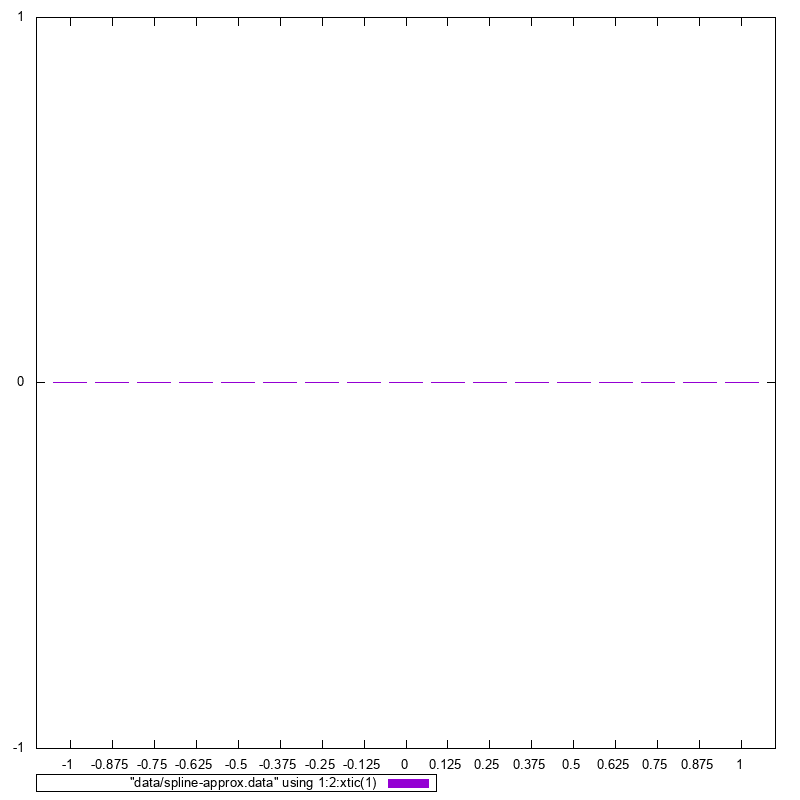
\includegraphics[width=0.4\textwidth]{spline-approx}
\end{figure}
Wat opvalt is dat de functie mooi door alle punten gaat! Dit is dan ook logisch omdat de spline feitelijk $2^{de}$ graads veeltermen genereert tussen de originele puntenkoppels.
\end{document}